\documentclass{article}
\usepackage[utf8]{inputenc}
\usepackage{authblk}
\usepackage{setspace}
\usepackage[margin=1.25in]{geometry}
\usepackage{graphicx}
\graphicspath{ {./figures/} }
\usepackage{subcaption}
\usepackage{amsmath}
\usepackage{lineno}
\usepackage{tikz-cd}
\usepackage[style=nejm, citestyle=numeric-comp, sorting=none]{biblatex}
\addbibresource{main.bib}

%%%%%% Document Setup %%%%%%

\title{6.4132/16.413 Principles of Autonomy and Decision Making Final Project}
\author[ ]{Toya Takahashi}
\affil[ ]{Massachusetts Institute of Technology}
\affil[ ]{Department of Aeronautics and Astronautics}
\onehalfspacing

%%%%%% Main Text %%%%%%

\begin{document}

\maketitle

\section{Introduction}

Activity planing, motion planning, and trajectory optimization for a robotic arm is challenging. To navigate around an environment, the agent must perform a state space search to plan a sequence of actions and generate a trajectory by either using a sample based planner or modeling the problem as a constraint optimization problem. This project explores 1) defining an activity planning problem with the Planning Domain Definition Language, 2) implementing the Fast-Forward heuristic planner with Enforced Hill Climbing, 3) using RRT with goal-biasing for trajectory generation, and 4) comparing the results with the trajectory generated by constraint optimization. The kitchen simulation environment provides an excellent sandbox for testing and demonstrating the effectiveness of the proposed approach, in addition to learning the benefits and drawbacks of the implemented algorithms.

\begin{figure}[h]
    \centering
    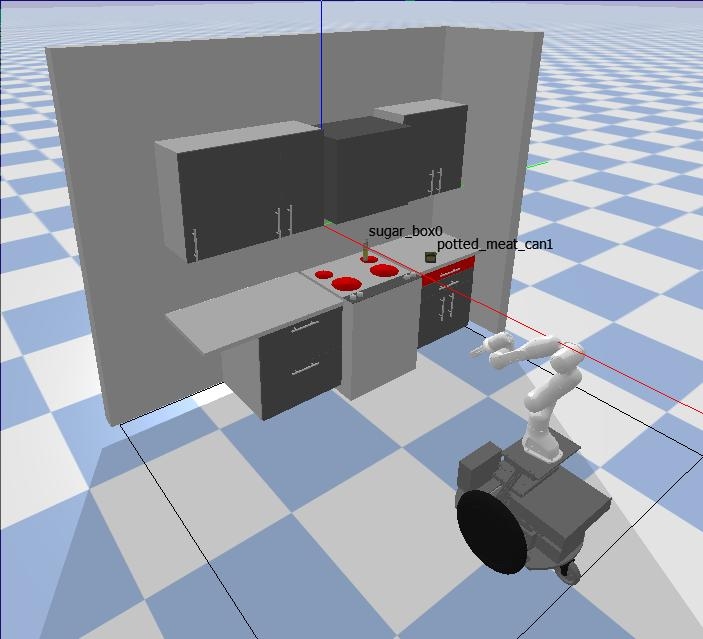
\includegraphics[width=190px]{sim_env.jpg}
    \caption{The kitchen simulation environment.}
    \label{fig:sim_env}
\end{figure}

\section{Activity Planning}

\iffalse
\subsection{Problem Statement}

The simulator consists of a kitchen environment with drawers, cabinets, countertops, and a robot manipulator arm. In addition, sugar and spam boxes are placed on a stovetop burner and a countertop. The objective is to move the sugar box to a nearby countertop and store the spam box inside the red drawer below it.

\begin{figure}[h]
    \centering
    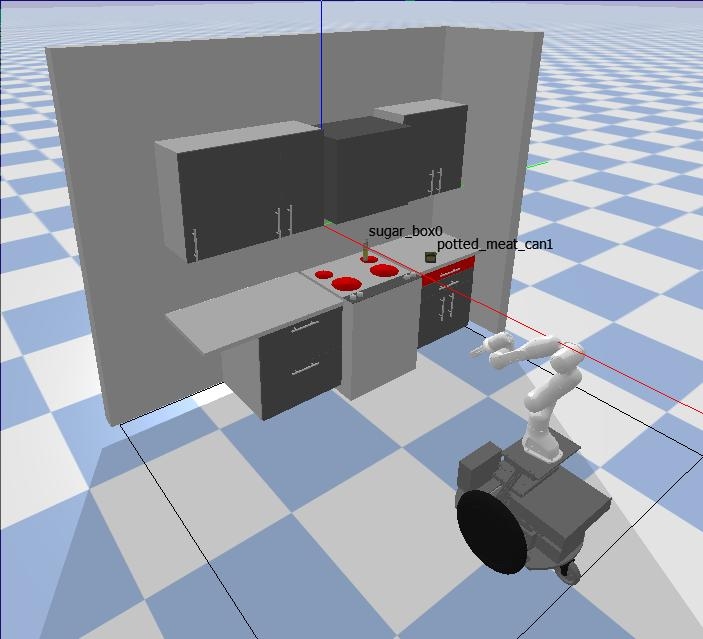
\includegraphics[width=200px]{sim_env.jpg}
    \caption{The kitchen simulation environment.}
    \label{fig:sim_env}
\end{figure}
\fi

\subsection{PDDL Domain and Problem}

The PDDL domain and problem files encode the problem as sets of objects, types, predicates, actions, and goals. There are two main types of objects: the \texttt{box} type and the \texttt{storage} type. The \texttt{box} type represents the sugar and spam boxes which are manipulated by the robot arm, and the \texttt{storage} type represents the storage spaces in the kitchen. In addition, I separated the \texttt{storage} type into two subtypes: \texttt{static}, which are storage spaces without actions (stovetop burner and countertop), and \texttt{openable}, which are storage spaces that can be opened or closed (drawer, cabinet).

The following assumptions were made when designing the actions and the initial state:
\begin{itemize}
    \item The robot can only grab one box at a time
    \item The robot cannot open drawers or cabinets when gripping an object
    \item Only one box can be placed on each storage space at a time
    \item Drawers and cabinets must be open when placing or picking up a box inside them
    \item Drawers and cabinets must be closed at both the beginning and end of the plan 
\end{itemize}

\begin{figure}[h]
    % https://q.uiver.app/#q=WzAsNSxbMSwwLCJcXHRleHR7b2JqZWN0fSJdLFswLDMsIlxcdGV4dHtzdG9yYWdlfSJdLFsyLDMsIlxcdGV4dHtib3h9Il0sWzAsNiwiXFx0ZXh0e3N0YXRpY30iXSxbMSw2LCJcXHRleHR7b3BlbmFibGV9Il0sWzEsMCwiXFx0ZXh0e2V4dGVuZHN9Il0sWzIsMCwiXFx0ZXh0e2V4dGVuZHN9IiwyXSxbNCwxLCJcXHRleHR7ZXh0ZW5kc30iLDJdLFszLDEsIlxcdGV4dHtleHRlbmRzfSJdXQ==
    \[\begin{tikzcd}
        & {\text{object}} \\
        \\
        \\
        {\text{storage}} && {\text{box}} \\
        \\
        \\
        {\text{static}} & {\text{openable}}
        \arrow["{\text{extends}}", from=4-1, to=1-2]
        \arrow["{\text{extends}}"', from=4-3, to=1-2]
        \arrow["{\text{extends}}"', from=7-2, to=4-1]
        \arrow["{\text{extends}}", from=7-1, to=4-1]
    \end{tikzcd}\]

    \caption{Hierarchical PDDL object types including static/openable storage spaces and boxes}
    \label{fig:types}
\end{figure}

Separating the \texttt{storage} type into subtypes allowed separating the action of placing (and picking up) a box on a storage space into \texttt{place\_static} and \texttt{place\_openable}, which has an extra \texttt{(open ?s)} precondition.

I also did not use any negative preconditions to simplify the implementation of the fast-forward heuristic planner. For actions requiring negative preconditions, I defined a second predicate which is always the negation of the predicate needing to express the negative precondition on (e.g. \texttt{(open ?s - openable)} and \texttt{(closed ?s - openable)}).

\subsection{Fast-Forward Heuristic Planner}

The \texttt{ff\_planner} file contains all functions to solve the activity planning problem. The \texttt{calculate\_hff} function computes the fast-forward heuristic $h_{ff}$ of a given state by counting the number of actions (without delete effects) it takes until the goal condition is a subset of \texttt{state}. At each iteration, \texttt{new\_state} is computed by taking the union of the current state and the add effects of all applicable actions. Because we defined our actions to only have positive preconditions, we can easily determine whether an action is applicable by checking if the precondition is a subset of \texttt{new\_state}. $h_{ff}$ is an admissible heuristic that always underestimates the number of actions it takes to reach the goal state, hence an alternative algorithm such as A* could have been used to find the optimal path.

In this project, I decided to implement Enforced Hill Climbing in the \texttt{solve\_ff} function. While EHC is not guaranteed to find the optimal solution, its greedy nature typically leads to higher efficiency and lower memory usage. \texttt{solve\_ff} initially parses the PDDL files and enumerates all possible actions that can be taken by the agent. Next, it performs a greedy search by immediately adding an action that leads to a strictly smaller $h_{ff}$ to the plan. If no such action is found, there is a ``plateau" in the graph, and BFS is used to find a sequence of actions that lead to a smaller $h_{ff}$. If BFS fails to find such action, then the algorithm determines that the activity planning problem is unsolvable.

Comparing the performance of BFS and FF Heuristic Planner, on the contrary to my expectation, I found that BFS consistently runs faster ($650\mu s$ vs. $950\mu s$). This is most likely because the plan graph is rather simple for this problem. For example, the starting state has $h_{ff}=2$, meaning EHC gets stuck on a ``plateau" for most of the time, resorting to BFS. In this case, calculating $h_{ff}$ leads to extra computation time. For more complex problems requiring many actions to be taken, I expect the FF Heuristic Planner to perform significantly faster than BFS.

\section{Motion Planning}

\section{Trajectory Optimization}

%%% TODO: EDIT REFERENCES %%%
\cite{Cui1}

\section{Conclusion}

\printbibliography

\end{document}
